% !Tex root = main.tex
\newpage
\section{Theory}

In this section, \emph{functional dependencies} (FDs) and the theoretical foundation necessary to put them into context, are introduced.
Common normal forms are briefly defined.
Building on this foundation, \emph{relaxed functional dependencies} are established as a way of adapting FDs for use-cases other than database normalization.

The term \emph{robustness} of FDs is discussed and defined.
A way of measuring robustness with cross-validation techniques is presented.
Lastly, machine learning classifier theory is reviewed, introducing \emph{Datawig Imputer}.

\subsection{Introduction of Functional Dependencies}
FDs are a way of expressing ``a priori knowledge of restrictions or constraints on permissible sets of data''.~\cite[p.~42]{MAI83}
In order to give a definition of FDs, they need to be put in context to the domain they stem from: relational database theory.

\paragraph{Definition (Relation Scheme, Attribute Names, Domain, Relation, Tuples)} A \emph{relation scheme}\footnote{also called \emph{relational schema} in literature\cite[p.21]{ABE19} } \(\boldsymbol{R}\) is a finite set of \emph{attribute names} \( \boldsymbol{R} = \{A_1,~A_2,~\dots,~A_n\}\), where to each attribute name \(A_i\) corresponds a set \(D_i\), called \emph{domain} of \(A_i\), \(1 \leq i \leq n\).
Let \(\boldsymbol{D}~=~D_1 \cup D_2 \cup \dots \cup D_n$, then a \emph{relation} \(r\) on relation scheme \(\boldsymbol{R}\) is a finite set of mappings \(\{t_1, t_2, \dots, t_p\}\) from \(\boldsymbol{R}\) to \(\boldsymbol{D}\):
\begin{align*}
  &t_i: \boldsymbol{R} \to \boldsymbol{D}
\end{align*}
We call those mappings \emph{tuples} under the constraint that~\cite[p.2]{MAI83}
\begin{align*}
    t(A_i) \subseteq D_i.
\end{align*}
In application, attribute names are commonly called \emph{column name} or \emph{column attribute}.
One can think of them as labels of data that is stored in the respective column.


\paragraph{Definition (Functional Dependency)}
Consider a relation \(r\) on scheme \(\boldsymbol{R}\) with subset \(X \subseteq \boldsymbol{R}\) and a single attribute \(A_i \in \boldsymbol{R}\).
A FD \(X \to A\) is said to be \emph{valid} in \(r\), if and only if
\begin{align}
    t_i[X] = t_j[X] \Rightarrow t_i[A] = t_j[A] \label{eq:fd-condition}
\end{align}
holds for all pairs of distinct tuples \(t_i,t_j \in r\).~\cite[p.~21]{ABE19}
We say that \textsc{X} \emph{functionally determines} \textsc{A}~\cite[p.~43]{MAI83} and write \textsc{X}~\( \rightarrow \)~\textsc{A}.
\(X\) is called the \emph{left hand side} (LHS) of a FD, whilst \(A\) is called the \emph{right hand side} (RHS) of the same FD.
A FD \textsc{X}~\( \rightarrow \)~\textsc{Y} is called \emph{trivial}, if \( Y \subseteq X \).\cite[p.~163]{STU16}

\paragraph{Example} Considering table~\ref{tab:fd-example}, one can see that every tuple in the left hand side subset of the relation uniquely determines the right hand side.
We say that \textsc{Id}, \textsc{Prenameame}, \textsc{Surname}, \textsc{Town} \emph{functionally determines} \textsc{Zip} or write \{\textsc{Id}, \textsc{Prename}, \textsc{Surname}, \textsc{Town} \}~\( \rightarrow \)~\textsc{Zip}.~\cite[p.~43]{MAI83}

\begin{table}[ht]
    \centering
    \begin{tabular}{rlllr}
        \toprule
        \toprule
        & \multicolumn{3}{c}{left hand side} & \multicolumn{1}{c}{right hand side} \\ \cmidrule(lr{.25em}){1-4} \cmidrule(l{4.75em}){4-5}
        \textsc{Id} & \textsc{Prename} & \textsc{Surname} & \textsc{Town} & \textsc{Zip} \\
        \midrule
        1 & Alice & Smith & Munich & 19139 \\
        2 & Peter& Meyer & Munich & 19139 \\
        3 & Ana & Parker & Munich & 19139  \\
        4 & John & Pick & Berlin & 12055 \\
        5 & John & Pick & Munich & 19139 \\
        \bottomrule
        \bottomrule
    \end{tabular}
    \caption{Example of a FD.}\label{tab:fd-example}
\end{table}

If inspected closely, one can discover even more FDs in table~\ref{tab:fd-example}.
For example, \textsc{Town}~\( \rightarrow \)~\textsc{Zip} and \textsc{Id}~\( \rightarrow \)~\textsc{Zip}.
Since \textsc{Town} and \textsc{Id} are subsets of \{\textsc{Id},~\textsc{Prename},~\textsc{Surname},~\textsc{Town}\}, we call the FD \{\textsc{Id},~\textsc{Prename},~\textsc{Surname},~\textsc{Town}\} \( \rightarrow \)~\textsc{Zip} \emph{non-minimal}.

\paragraph{Definition (Minimal FD)} A FD X~\( \rightarrow \)~A is \emph{minimal}, if no subset of X functionally determines A.~\cite[p.~2]{PAP15}
Thus, \textsc{Id}~\( \rightarrow \)~\textsc{Zip} and \textsc{Town}~\( \rightarrow \)~\textsc{Zip} are \emph{minimal FDs}.

\paragraph{Definition (Logical Implication)} Let \( F \) be the set of FDs on \( \boldsymbol{R} \).
\textsc{X}~\( \rightarrow  \)~\textsc{Y} is \emph{logically implied} by \( F \), or algebraically expressed
\begin{align}
    F \models \textsc{X} \rightarrow \textsc{Y},
\end{align}
if every relational instance \( r \) of \( \boldsymbol{R} \), which satisfies all dependencies in \( F \), also satisfies \textsc{X}~\( \rightarrow \)~\textsc{Y}.~\cite[p.~166]{STU16}

Thus, if \( F = \{ \textsc{A} \rightarrow \textsc{B},~\textsc{A} \rightarrow \textsc{C},~\textsc{BC} \rightarrow \textsc{D} \} \), the following logical implications are true:
\begin{align*}
    &F \models \textsc{A} \rightarrow \textsc{B} \\
    &F \models \textsc{A} \rightarrow \textsc{BC} \\
    &F \models \textsc{A} \rightarrow \textsc{D}
\end{align*}

\paragraph{Definition (Transitive Closure)} Let \( F \) be a set of FDs.
The \emph{transitive closure} \( F^{+} \) of \( F \) is defined by
\begin{align}\label{eq:transitive-closure}
    F^{+} := \{ \textsc{X} \rightarrow \textsc{Y} \mid F \models \textsc{X} \rightarrow \textsc{Y} \}
\end{align}

\paragraph{Definition (Full Dependency, Determinant)} Let \( \mathbf{R} \) be a relation scheme and let \( \textsc{Y} \in \mathbf{R} \) be an attribute on \( \mathbf{R} \).
Furthermore, let \( \textsc{X} \subseteq \mathbf{R} \) be a set of attributes on \( \mathbf{R} \).
The attribute \textsc{Y} is called \emph{fully dependent} on \textsc{X}, if \textsc{Y} is functionally determined by \textsc{X} and \textsc{X} is minimal.~\cite[p.~61]{SCH17}
We call a \emph{determinant} a set of attributes that fully functionally determines another attribute.

\subsection{Additional Relational Database Theory}
When real-world data used by an application is stored on a machine according to the relational model, it is usually stored in a relational database.
\emph{Database normalization} is the original domain of application for FDs.~\cite[p.~381]{COD70}
In the following section, concepts necessary for introducing databases are defined.
In addition, terms used in database normalization are defined.

\paragraph{Definition (Superkey)}Let \( r \) be a relation and let \( \boldsymbol{R} = \{ A_1, A_2, \dots, A_n \},~n \in \mathbb{N} \), be a relation scheme on which \( r \) is defined.
Let \( K \) be a subset of R, such that \(K = \{ A_1, A_2, \dots, A_m \} \subseteq \boldsymbol{R} \), where \( m \leq n,~m \in \mathbb{N} \).
The subset \( K \) is called \emph{superkey}, if for any tuple \( t_i \in r \) the relation
\begin{align*}
    t_i(A_k) = t_j(A_k) \Rightarrow t_i \equiv t_j
\end{align*}
holds for any single \( A_k \in K \).~\cite[p.~4]{MAI83}
In other words, if \( K \) is a superkey, any \( K \)-value of a tuple identifies that tuple uniquely.~\cite[p.~32]{SCH17}

\paragraph{Definition (Candidate Key)} A superkey \( K \) is called \emph{candidate key}, if it is \emph{minimal}.~\cite[p.~32]{SCH17}
The notion of \( K \) being minimal means that \( K \) is no longer a superkey, if any attribute \( A_k \in K \) is removed from \( K \).

\paragraph{Definition (Prime Attributes)} An attribute \( A \) on a relational scheme \( \boldsymbol{R} \) is called \emph{prime}, if \( A \) is part of a key of \( \boldsymbol{R} \).
Otherwise, \( A \) is called \emph{non-prime}.

\paragraph{Definition (Relational Database)}
Following the definition of a relation scheme \( \boldsymbol{R} \), one can formally introduce databases and database schemes:

We assume that \( \boldsymbol{R}\) is composed of two parts, \(S\) and \(\boldsymbol{K}\). We call \(S\) a \emph{set of attributes} and \(\boldsymbol{K}\) a \emph{set of designated keys} and describe this composition by writing \(R = (S, \boldsymbol{K})\).
A \emph{relational database scheme} \( \mathcal{R} \) over \( \boldsymbol{U} \) can now be defined as a collection of relation schemes \( \mathcal{R} = \{R_1, R_1, \dots, R_p\} \), where \(R_i = (S_i, \boldsymbol{K}_i)\), \(1 \leq i, j \leq p\),
\begin{align*}
    \boldsymbol{U} := \bigcup^{p}_{i=1} S_i
\end{align*}
We demand that \(S_i \neq S_j\) if \(i \neq j\).

A \emph{relational database} \( d \) on a \emph{database scheme} \( \mathcal{R} \) is a collection of relations \( d~=~\{r_1, r_2, \dots, r_p \} \) such that for each relation scheme \(R = (S, \boldsymbol{K}) \) in \( \mathcal{R} \) there is a relation \(r\) in \(d\) such that \(r\) is a relation on \(S\) that satisfies every \emph{key} in \(\boldsymbol{K}\).~\cite[p.~94]{MAI83}


\subsection{Database Normalization}
In 1970, Edgar F. Codd defined the \emph{relational model}~\cite{COD70} and pioneered many important concepts in database theory.
When introducing the relational database model in his 1970 article ``A relational model of data for large shared data banks'', Codd formalized database normalization alongside.~\cite{COD70}

Describing what will be know to academia as \emph{First Normal Form} (1NF), Codd states that ``problems treated [when normalizing databases] are those of \emph{data independence}'', aiming to protect future users of large databases ``from having to know how the data is organized in the machine''.~\cite[p.~1]{COD70}

Databases at the time were structured hierarchically or navigationally.
This design was centered on efficiency, optimized for handling queries as fast as possible.
While this design yielded good performance in an era when computing time was cost-intensive, it came with a heavy cost of complexity:
``Teams of programmers were needed to express queries to extract meaningful information. [\dots] Such databases [\dots] were absolutely inflexible[y]''.~\cite{IBM03}

Codd's relational model shifted the focus of database architecture away from efficiency towards a new design, centered around the user of a database.
However, this new approach of database architecture came with new challenges.
How does one create a database-scheme with favorable properties?

Generally, redundantly stored data is an indicator~\cite[p.~61]{WAT14} that so-called \emph{anormalies} might occur, leading to inconsistency when operating the database.~\cite[p.~162]{STU16}
Kleuker writes that ``with a certain `database-sense'\ '' one could sense when splitting tables up is necessary to prevent anormalies.~\cite[p.~76]{KLE11}

This `database-sense' was formalized when Codd introduced database normalization as part of the relational model.~\cite[p.~381]{COD70}
Different \emph{normal forms} were defined.
Codd used three normal forms, which he called First-, Second- and Third Normal Form.\footnote{The Third Normal Form was later newly formulated by Boyce and Codd and named Boyce-Codd Normal Form (BCNF). Due to its more elegant definition, BCNF is introduced rather than Codd's original 3NF.}

Subsequently, Fourth-, Fifth- and even higher-order Normal Forms were defined by other authors.
However, these normal forms find little reception in real-world applications.~\cite[p.~58]{SCH17}
Today, FDs are primarily used in database normalization.~\cite[p.~1]{CAR16}
Thus, the derivation of the most commonly used normal-forms is of interest within the scope of this work.

\paragraph{Definition (First Normal Form)} A relation scheme $R$ is in \emph{First Normal Form} (1NF), if values in \(dom(A)\) are atomic for every attribute \(A \in R\).~\cite[p.~96]{MAI83}
Likewise, a database scheme \textbf{R} is in 1NF if every relation scheme \(R \in \textbf{R} \) is in 1NF.\

\paragraph{Example}Consider table~\ref{tab:first-normal-form} which represents two relational instances on two different relational schemes.
It serves as an example of what is called atomic- and compound data in the Relational Database model.~\cite[p.~6]{COD90}

\begin{table}[ht]
    \centering
    \ra{1.3}
    \begin{tabular}{rlllllll}
        \toprule
        \toprule
    & \multicolumn{3}{c}{Compound Scheme} & & \multicolumn{2}{c}{Atomic Scheme} \\
    \cmidrule{2-3} \cmidrule{5-8}
    & \textsc{Name} & \textsc{Adress} && \textsc{Prename} & \textsc{Surname} & \textsc{Town} & \textsc{Street}   \\ \midrule
1 & Alice Smith & Munich, Flurstr. && Alice & Smith & Munich & Flurstr. \\
2 & Peter Smith & Munich, Flurstr. && Peter & Smith & Munich & Flurstr. \\
3 & Ana Parker & Munich, Anastr. && Ana & Parker & Munich & Anastr. \\
4 & John Pick & Berlin, Flurstr. && John & Pick & Berlin & Flurstr. \\
\bottomrule
\bottomrule
\end{tabular}
\caption{The compound attributes \textsc{Adress} and \textsc{Name} can be split into their atomic components \textsc{Town} and \textsc{Street} as well as \textsc{Prename} and \textsc{Surname}, respectively.}\label{tab:first-normal-form}
\end{table}
Note that the compound scheme's attributes can be decomposed into several other attributes.
The atomic scheme's attributes however cannot be further split into any meaningful smaller components.

1NF is the very foundation of the Relational Model. It demands, that the only type of compound data is the relation itself.~\cite[p.~6]{COD90}

\paragraph{Definition (Second Normal Form)} A relation scheme \(R\) is said to be in \emph{Second Normal Form} (2NF) in respect to a set of FDs \(F\), if it is in 1NF and every nonprime attribute is fully dependent on every key of \(R\).~\cite[p.~99]{MAI83}
This definition can be extended for databases: A database scheme \textbf{R} is in 2NF with respect to \(F\) if every relation scheme \(R \in \textbf{R} \) is in 2NF with respect to \(F\).

It can be shown that a database scheme in 2NF is also in 1NF.~\cite[p.~58]{SCH17}

\paragraph{Definition (Boyce-Codd Normal Form)}
A relation scheme \( R \) is in \emph{Boyce-Codd Normal Form} (BCNF), if every determinant in \( R \) is a candidate key.~\cite[p.~65]{SCH17}
Equally, a relational database scheme \( \textbf{R} \) is in BCNF if every relation scheme \( R \in \textbf{R} \) is in BCNF.\

If a database scheme is in BCNF, it is also in 2NF.~\cite[p.~58]{SCH17} A database in BCNF effectively eliminates redundancies apart from candidate keys, freeing a database in BCNF from anormalies.~\cite[p.~67]{SCH17}


\subsection{Relaxed Functional Dependencies}
When Edgar F. Codd introduced the relational model in 1970, the concept of keys and thus the concept of FDs was already present.~\cite[p.~70]{MAI83}
However, in 1972 Codd separated the definition of a FD from keys, persuing the specific goal of normalizing a relational database scheme.

In the ensuing time, researchers abstracted the concept of FDs and transferred the approach.
FDs were used in research to solve problems other than schema normalization.~\cite[p.~161]{CAR16}
Many of these use-cases, such as `approximate classification' or `source merging', arose due to the fact that real-world datasets are almost always \emph{noisy}.

Noise in databases has many faces:
Entries might be corrupted by missing data, wrongly entered data or incomplete data.
A database might have been merged with identical entries formatted in different ways.~\cite[p.~1]{KOU09}
In these cases, functionally dependent column-combinations are not detected as such by a FD detection algorithm searching for FDs as defined in~\ref{eq:fd-condition}.
This may result in misleading insights when searching for FDs or normalizing a database.

Taking these limitations of \emph{canonical FDs}\footnote{To accentuate the difference between FD and RFD, FDs are also called canonical FDs. This notion refers to FDs as defined in equation~\ref{eq:fd-condition}.} into account, a multitude of new dependencies was defined, ``aiming to solve specific problems''.~\cite[p.~147]{CAR16}
Since all of these new kinds of dependencies \emph{relax} the conditions in equation~\ref{eq:fd-condition}, they are called \emph{relaxed functional dependencies} (RFDs).

Caruccio et al.\ classified and compared 35 different RFDs.~\cite[p.~151]{CAR16}
They state that each RFD was ``based on its underlying relaxation criteria''.~\cite[p.~149]{CAR16}
They proceed to define two relaxation criteria by which they distinguish all RFDs.

\begin{figure}[ht]
     \centering
     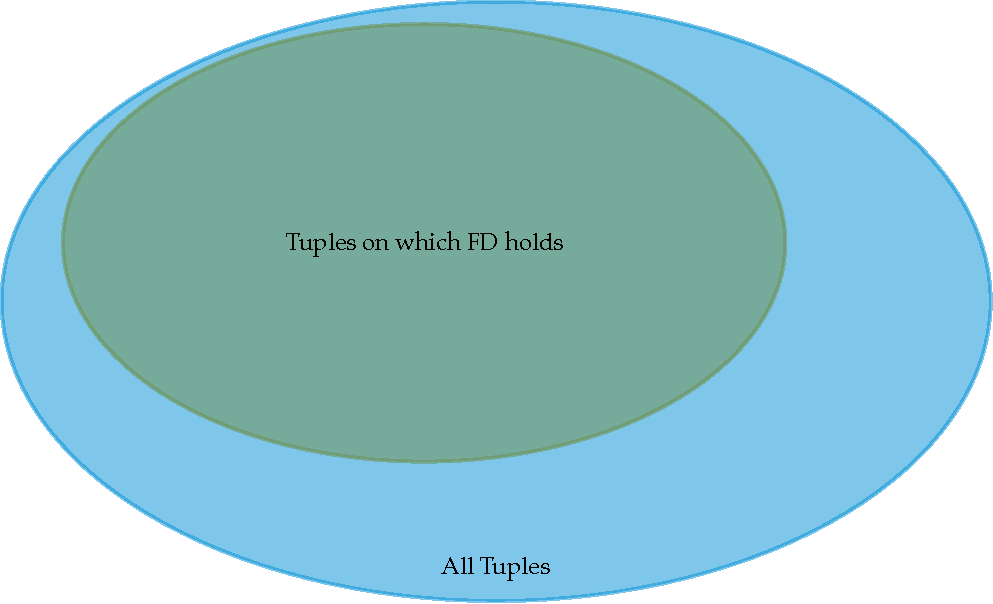
\includegraphics[width=\textwidth]{images/rfds-extent.pdf}
     \caption{Venn diagram representing the extent relaxation criterion.}
     \label{fig:rfds-extent}
 \end{figure}

The first relaxation criterion is called \emph{attribute comparison}.
It refers to ``the type of tuple comparison used on the LHS and RHS'' in equation~\ref{eq:fd-condition}.

The relaxation criterion \emph{extent} implies a relaxation of the set of tuples for which a FD is valid.

\subsubsection{FDs relaxing on the Extent}
The term \emph{extent} is used to describe how a RFD relaxes on the subset of tuples for which the RFD is satisfied.
While the definition of a FD demands that a FD's condition has to be valid for all tuples in a relational table, RFDs relaxing on the extent only hold on a subset of all tuples.

This idea is implemented by different RFDs in different ways.
In the following section, a selection of RFDs relaxing the extent of the FD is briefly presented.

\paragraph{Approximate Functional Dependency (AFD)}
AFDs improve the applicability of FDs by ``holding on \emph{almost}\footnote{Highlighting by the author.} every tuple''\cite[p.~151]{CAR16}.
To illustrate this, table~\ref{tab:example-afd-necessity} shows an example of noisy data.
The potential FD \textsc{Town}~\(\to\)~\textsc{Zip} is not captured by the definition of a canonical FD.\
Due to a typing error, the potential FD is invalidated in the row where \textsc{ID = 2}.
To still capture the relation, a different dependency-measure than given in the definition of the canonical FD is required.

\begin{table}[ht]
    \centering
    \begin{tabular}{lcccc}
        \toprule
        \toprule
        \textsc{Id} & First name & Last name & Town & \textsc{Zip} \\
        \midrule
        1 & Alice & Smith & Munich & 19139 \\
        \textbf{2} & \textbf{Peter}& \textbf{Meyer} &
        \textbf{Muinch} & \textbf{19139} \\
        3 & Ana & Parker & Munich & 19139  \\
        4 & John & Pick & Berlin & 12055 \\
        \bottomrule
        \bottomrule
    \end{tabular}
    \caption{Even though column \textsc{Zip} determines the content of column \textsc{Town}, a FD is not capable of displaying this fact due a typing error in column \textsc{Town}.}
    \label{tab:example-afd-necessity}
\end{table}

Tuples that do not correspond to the canonical FD are measured as fraction of the total of tuples on a relation \( r \) as follows:

\begin{align}
    \Psi(X, Y) = \frac{\min{\left(|r_1|~|~r_1 \subseteq r \text{ and } \textsc{X} \rightarrow \textsc{Y} \text{ hold in } r \setminus r_1 \right)}}{|r|}
\end{align}

Here, function \( \Psi(X, Y) \) is called \emph{coverage measure} of a RFD \textsc{X} \( \to \) \textsc{Y}.
\( \Psi \) ``quantifies the satisfiability degree of an RFD [\dots] on \( r \)''~\cite[p.~150]{CAR16} and is used in the definition of an AFD to be compared to a threshold \( \epsilon \in [0, 1] \).

If \( \Psi(X, Y) \) is smaller or equal to \( \epsilon \), the AFD is said to hold on a relation \( r \).
Applied to table~\ref{tab:example-afd-necessity}, the AFD \textsc{Town} \( \to \) \textsc{Zip} holds, if \( \epsilon \geq 0.25\).

\paragraph{Conditional Functional Dependencies (CFDs)}
\emph{Conditional Functional Dependencies} employ conditions to define the subset on which a dependency holds.
Originally, those conditions exclusively allow the definition of constraints using the equality operator.~\cite[p.~152]{CAR16}
Applied to table~\ref{tab:example-afd-necessity}, a CFD \textsc{Town} \( \to\) \textsc{Zip} holds under the condition that a) entries in column \textsc{Town} = Munich or b) entries in column \textsc{Town} = Berlin.

Other RFDs based on the definition of CFDs include \emph{extended conditional functional dependencies} (ECFDs) by Bravo et al.\ that allow the disjunction-operator as well as the inequality-operator for defining conditions.~\cite{BRA08}

Also, Chen et al.\ defined CFD\textsuperscript{p}s, which introduce \( <, \leq, >, \geq \text{and} \neq \) for defining conditions.~\cite{CHE09}

\subsubsection{FDs Relaxing on the Attribute Comparison}
Instead of specifying subsets of tuples for which a FD is valid, FDs relaxing on the attribute comparison alter the condition under which a dependency is said to be valid.
One common RFD relaxing on the attribute comparison is the metric functional dependency.

\paragraph{Metric Functional Dependencies (MFDs)}
First introduced by Koudas et al.\ in 2009, \emph{Metric Functional Dependencies} were defined to adress violations of canonical FDs due to ``small variations [\dots] in data format and interpretation''.~\cite[p.~1]{KOU09}

According to equation~\ref{eq:fd-condition}, a FD \textsc{Zip} \( \to\) \textsc{Town} is said to be valid if
\begin{align}
    t[\textsc{Zip}] = t'[\textsc{Zip}] \Rightarrow t[\textsc{Town}] = t'[\textsc{Town}]
\end{align}
holds for all pairs of distinct tuples \( t_i, t_j \in r \), where \( r \) is a relation on scheme \( \boldsymbol{R} \).
The definition of a MFD replaces this equation by demanding that if and only if for all pairs of distinct tuples \( t_i, t_j \in r \) the metric condition
\begin{align}\label{eq:mfd-condition}
    t[\textsc{Zip}] = t'[\textsc{Zip}] \Rightarrow d(t[\textsc{Town}], t'[\textsc{Town}]) \leq \delta
\end{align}
holds, the MFD \textsc{Zip} \( \to\) \textsc{Town} is said to be valid on \( r \).~\cite[p.~2]{KOU09}
Here, \( \delta \) is called a \emph{tolerance parameter}, indicating how far the result of a \emph{metric} \( d(t[\textsc{Y}], t'[\textsc{Y}]) \) can deviate from exact equality.

One such metric \( d \) would be the absolute difference between two values, such that \( d(t[\textsc{Y}], t'[\textsc{Y}]) = | t[\textsc{Y}] - t'[\textsc{Y}]| \).
Another popular metric for measuring the difference between two sequences is the Levenshtein distance, where \( d(t[\textsc{Y}], t'[\textsc{Y}]) = \text{lev}_{t,t'}(|t|, |t'|) \) and
\begin{align*}
    \text{lev}_{t,t'} =
    \begin{cases}
        \max(i,j),  & \text{if} \min(i,j)=0, \\
        \min \begin{cases}
            \text{lev}_{a, b}(i-1, j)+1 & \\
            \text{lev}_{a, b}(i, j-1)+1 & \\
            \text{lev}_{a, b}(i-1, j-1)+1_{(a_i \neq b_j)} \\
        \end{cases} & \text{otherwise.}
    \end{cases}
\end{align*}
Regarding the example given in table~\ref{tab:example-afd-necessity}, the Levenshtein distance between \texttt{Munich} and \texttt{Muinch} is 2.
Thus the MFD \textsc{Zip} \( \to\) \textsc{Town} is valid, if \( d = \text{lev} \) and \( \delta = 2 \).

\subsection{Robustness of FDs}
Koudas et al., when introducing the MFD, write that the definition of the canonical FD was ``not \emph{robust} enough to capture functional relationships on data obtained from merging heterogenous sources [\dots]''\footnote{Highlighting added by the author.}.~\cite[p.~1]{KOU09}
However, they do neither provide a definition of robustness, nor a way to measure it.

Bleifuß et al.~\cite[p.~3]{BLE16} define a measure similar to robustness called \emph{Correctness}.
They do so by comparing a set of RFDs \( Out \) to a set of FDs \( Gold \) on the same relational instance \( r \) as follows:
\begin{align*}
    \text{Correctness} = \frac{|Out \cap Gold^{+}|}{|Out|}
\end{align*}
\( Gold^{+} \) represents the transitive closure of \( Gold \), meaning that it includes all non-minimal FDs implied by \( Gold \) as defined in equation~\ref{eq:transitive-closure}.

By this definition, the notion `Correctness' considers \( Out \) to be more or less `correct' depending on how many members it has in common with \( Gold^{+} \).
If a RFD is used to find relations on noisy data, this definition of `Correctness' does not meaningfully measure dependencies that try to work around the noise.
This means that a RFD that takes the typing error in table~\ref{tab:example-afd-necessity} into account would not be more `correct' than a RFD that does not.

In summary, Koudes et al.\ do not provide a definition of robustness and `Correctness' cannot be used for measuring robustness.
Drawing inspiration from Machine Learning theory, the application of cross-validation techniques to FDs order to measure robustness is proposed.

\paragraph{Definition (Train Set, Test Set, Split Ratio)} Let \( r = \{ t_1, t_2, \dots, t_p \}\) be a  relation on a relation scheme \( \boldsymbol{R} \) where \( p \in \mathbb{N} \) is the number of tuples in \( r \).
Let \( s \in [0, 1] \) be the \emph{split ratio} and let \( m = \lfloor s \cdot p \rfloor \), then we define:
\begin{align}
    r_{train} &= \{ t_1, t_2, \dots, t_{m} \} \\
    r_{test} &= \{ t_{m + 1}, t_{m + 2}, \dots, t_{p} \},
\end{align}
such that \( r =  r_{train}~\dot\cup~r_{test} \) is split into two disjunct subsets.
We call \( r_{train} \) the \emph{train set} and \( r_{test} \) the \emph{test set}.\footnote{The naming `test set' is ambiguous in literature. Bishop~\cite{BIS06} and Smola et al.\ \cite{SMO08} call `validation set' what is called `test set' by Burkov~\cite[ch.~5, p.~8-9]{BUR19}. In this work, the notation from~\cite{BUR19} is adopted.}~\cite[p.~56]{SMO08}

\paragraph{Definition (Imputation Derived by a FD)}
Let \( r \) be a relational instance on a relational scheme \( \mathbf{R} \).
In addition, let \( \textsc{X} \subseteq \mathbf{R} \) and \( \textsc{A} \in \mathbf{R} \), \( \textsc{A} \notin X\).
Furthermore, let \textsc{X}~\( \rightarrow \)~\textsc{A} be a non-trivial, minimal FD of \( r_{train},~r = r_{train}~\dot\cup~r_{test} \).
For all tuples \( t \in r_{train} \) where
\begin{align}\label{eq:fd-imputation}
    t[\textsc{X}] = t^{\prime}[\textsc{X}],
\end{align}
we call the RHS \( t[\textsc{A}] \) the \emph{imputation} of \( t^{\prime} \in r_{test} \) derived by the FD \( \textsc{X} \rightarrow \textsc{A} \).

\paragraph{Definition (Set of Imputations)}
Let \( r \) be a relational instance on a relational scheme \( \mathbf{R} \).
Moreover, let \( \textsc{X} \subseteq \mathbf{R} \) and \( \textsc{A} \in \mathbf{R} \), \( \textsc{A} \notin X\).
Also, let \textsc{X}~\( \rightarrow \)~\textsc{A} be a non-trivial, minimal FD of \( r_{train} \), where \( r = r_{train}~\dot\cup~r_{test} \).
We then call
\begin{align}
    r_{imp}^{i} = \big\{ t[A] \mid t[\textsc{X}] = t^{\prime}_{i}[\textsc{X}],~t^{\prime}_{i} \in r_{test},~t \in r_{train} \big\}
\end{align}
\emph{set of imputations} of the \( i \)th tuple in the test set.

\paragraph{Definition (Robustness)}
Let \( r = \{ t_1, t_2, \dots, t_p \}\) be a relational instance on a relational scheme \( \mathbf{R} \), \( p \in \mathbb{N} \).
Moreover let \( \textsc{X} \subseteq \mathbf{R} \) and \( \textsc{A} \in \mathbf{R} \), \( \textsc{A} \notin X\).
Let \textsc{X}~\( \rightarrow \)~\textsc{A} be a non-trivial, minimal FD of \( r_{train} \).
Furthermore, let \( r = r_{train}~\dot\cup~r_{test} \) be split with split ratio \( s \in [0, 1] \) and let \( m = \lfloor s \cdot p \rfloor \).

For each tuple \( t^{\prime}_i \in r_{test} \), let \( r^{i}_{test} \) be the set of imputations with regard to \textsc{X}~\( \rightarrow \)~\textsc{A}.
For all \( r^{i}_{test} \neq \emptyset \), we arbitrarily choose one tuple \( t_{imp}^{i} \) from \( r_{imp}^i \).
We call
\begin{align}\label{eq:imputation-set}
    r_{imp} = \big\{ t_{imp}^{i} \mid i \in \{ m + 1, m + 2, \dots, p \} \big\}
\end{align}
set of imputations of the test split.

Treating the tuples in \( r_{imp} \) as predicted labels and the tuples in \( r_{test} \) as labels, we compute the F1-Score or the MSE, depending on the type of data the RHS contains.
We call this Score `Robustness' of FD \textsc{X}~\( \rightarrow \)~\textsc{A}.


\subsection{FD Imputer: Measuring Robustness}
In table~\ref{tab:split-example-fd-imputer} a splitting is examplified for \( s = 0.5 \) and \( p=4 \).
The approach and terminology involved in the definition of robustness are based on methods from statistical cross-validation used in model selection~\cite[p.~172]{HAY08}.
When measuring robustness, FDs are first detected on the train set using a FD detection algorithm.
In this work, the HyFD algorithm is chosen.~\cite{PAP16}
The algorithm called \emph{FD Imputer} is then used for measuring robustness of each FD detected on the train set.

\begin{table}[ht]
    \begin{subtable}[c]{0.9\textwidth}
        \centering
        \begin{tabular}{llll}
            \textsc{A} & \textsc{B} & \textsc{C} & \textsc{D} \\
        \toprule
        \toprule
        Blue & Car & Portugal & Lisbon \\
        Yellow & Car & Portugal & Lisbon  \\
        Green & Bus & Spain & Madrid  \\
        Grey & Car & Portugal & Lisbon  \\
        \bottomrule
        \bottomrule
        \end{tabular}
        \subcaption{Original relation \( r \).}
    \end{subtable}
    \begin{subtable}[c]{0.45\textwidth}
        \centering
        \begin{tabular}{llll}
            \textsc{A} & \textsc{B} & \textsc{C} & \textsc{D}  \\
        \toprule
        \toprule
            Green & Bus & Portugal & Lisbon \\
            Yellow & Car & Portugal & Lisbon \\
        \bottomrule
        \bottomrule
        \end{tabular}
        \subcaption{Train set \( r_{train} \).}
    \end{subtable}
    \begin{subtable}[c]{0.45\textwidth}
        \centering
        \begin{tabular}{llll}
        \textsc{A} & \textsc{B} & \textsc{C} & \textsc{D} \\
        \toprule
        \toprule
        Yellow & Bus & Spain & Madrid \\
        Blue & Bus & Portugal & Lisbon \\
        \bottomrule
        \bottomrule
        \end{tabular}
        \subcaption{Test set \( r_{train} \).}
    \end{subtable}
    \caption{The relation \( r \) is split into train- and test sets with a split-ratio \( s = 0.5 \). }
    \label{tab:split-example-fd-imputer}
\end{table}

\paragraph{FD Imputer} FD Imputer iterates over all tuples in the test set and searches for a tuple in the train set with the exact same LHS.
If one or more such tuples in the train set are found, FD Imputer randomly selects one of these tuples and saves the RHS of that tuple.
As defined in the previous section, this RHS value is called \emph{imputation} of the RHS value on the train set.

This procedure is repeated for all tuples in the train set.
In a last step, FD Imputer compares the imputations with the actual RHS values in the train set.
This allows a classification of the imputations.
If the FD's RHS contains categorical data, one can now calculate the F1-measure for each FD.
Elsewise, in case the FD's RHS contains sequential data, the MSE is chosen as measure of robustness.

Consider table~\ref{tab:split-example-fd-imputer}.
The FD \textsc{C} \( \ \to \) \textsc{D}, when used for finding a right hand side value on \( r_{test} \), will correctly return `Lisbon'.
However, FD \textsc{A} \( \to \) \textsc{D} for example will lead to FD Imputer yielding `Madrid', which is an incorrect imputation.

The implementation of FD Imputer leverages SQL join clauses to retrieve imputations.
FD Imputer performs an inner join on all LHS columns, joining train-set and test-set.
A successive second left join clause concatenates the original test-set with the column of imputed tuples stemming from the first join.
The result is a set of imputations as described in equation~\ref{eq:imputation-set}.

\paragraph{Robustness as a F1-Score} The imputed values retrieved by FD Imputer can be leveraged to create a measure for robustness.
First, each imputed value is interpreted as a label.
These labels are then each classified as in the binary classification case (see figure~\ref{fig:confusion-matrix}).
Next, precision and recall are calculated and the F1-Score is derived according to equation~\ref{eq:f1-score}.

Lastly, the F1-Score weighted according to the number of true instances for each label is calculated.\footnote{See \href{https://scikit-learn.org/stable/modules/generated/sklearn.metrics.f1_score.html}{sklearn documentation} for \texttt{sklearn.metrics.f1\_score()} with weighted average for more details on the implementation.}

Algebraically, this means that to a set \( L = \{ l_1, l_2, \dots, l_n \} \) of \( n \in \mathbb{N} \) labels, a set \( X = \{ x_1, x_2, \dots, x_n \}\) of \( n \) F1-Scores corresponds.
Let \( W \) be a set of weights \( W = \{ w_1, w_2, \dots, w_n \} \), each being the number of true instances for each label.
Then the weighted F1-Score of a dependency can be calculated as follows:
\begin{align}\label{eq:fd-imputer-f1-score}
    \text{F1-Score} = \frac{\sum_{i=1}^{n} x_i w_i}{\sum_{i=1}^{n}w_i}
\end{align}
This F1-Score, calculated for each FD on a relation \( r \), is named robustness of a FD.

\paragraph{Robustness as Mean Squared Error}
Depending on the kind of data imputed by FD Imputer, the measure used to express robustness is adapted.
As shown in the previous paragraph, performance when imputing categorical data can be measured by the F1 Score.
If the RHS's content is of a sequential datatype, using a classification performance measure is pointless.

Therefore, FD Imputer distinguishes between sequential and categorical data.
When imputing sequential data, the \emph{mean squared error} (MSE) is chosen as measure.

Let \( \hat{Y} \in \mathbb{R}^{n}\) be the \( n \)-dimensional vector of imputed values and \( \hat{Y} \in \mathbb{R}^{n} \) be the vector of actual RHS values.
Then the MSE is defined as~\cite[p.~597]{MOO11}
\begin{align}\label{eq:fd-imputer-mse}
\text{MSE} = \frac{1}{n}\sum_{i=1}^{n} \left(Y_i - \hat{Y}_i\right)^2
\end{align}

\newpage

\subsection{Machine Learning Classifier Theory}
Once a model has been trained and validated, it needs to be tested in order to determine whether or not overfitting occured during training.~\cite[p.~32]{BIS06}
This is usually done by measuring the model's performance on a separate dataset not involved in training, the so called test set \( X_{test} \).
Performance is measured according to the type of data and the kind of model involved.
To visualize the performance of a classifier, a \emph{confusion matrix} can be created.~\cite[p.~2]{THA18}
\begin{figure}[ht]
     \centering
     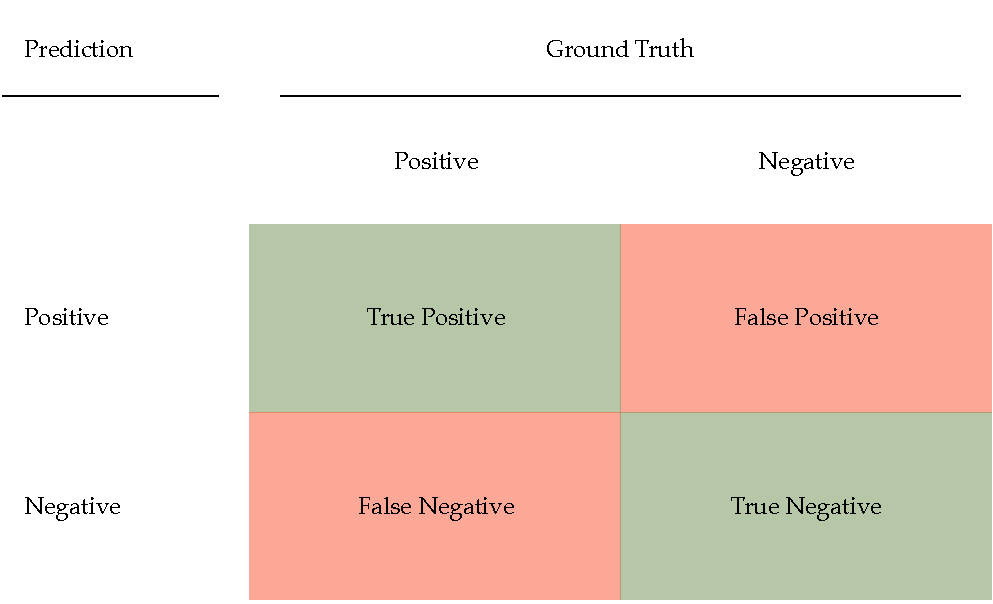
\includegraphics[width=\textwidth]{images/binary-confusion-matrix.pdf}
     \caption{Illustration of a binary confusion matrix.
     `Prediction' refers to predicted labels \(y_{pred}(x)\) while `Ground Truth' represents the actual labels \(y(x)\).}
     \label{fig:confusion-matrix}
 \end{figure}

 The simplest case of a confusion matrix can be constructed when measuring the performance of a binary classifier.
Figure~\ref{fig:confusion-matrix} shows such a \( 2 \times 2 \) binary confusion matrix.
Here, `Ground Truth' describes the label \(y(x)\) of some data point \(x \in X_{test}\), where \(y \in \{0, 1\}\).
`Prediction' identifies the predicted labels \(y_{pred}(x)\) that the model generates after is has been executed on the test-set \(X_{test}\) prior unknown.

Whenever \(y_{pred}(x) = y(x),~x \in X_{test}\) holds, the predicted label can be assigned to be either a \emph{True Positive} (TP) or a \emph{True Negative} (TN).
The opposite holds as well, such that a falsely predicted label will be either a \emph{False Negative} (FN) or a \emph{False Positive} (FP).~\cite[p.~2]{THA18}

Using the classification introduced by the binary confusion matrix, all predicted labels \(y_{pred}\) are assigned to the four sets TP, TN, FN and FP.
Using these four sets, we can introduce measures for classification performance.

\emph{Precision} is a measure that depicts the proportion of correctly classified positive samples to the total amount of samples classified as positive.\cite[p.~4]{THA18} This can be algebraically expressed as
\begin{align}\label{eq:precision}
    Precision = \frac{|TP|}{|TP| + |FP|}
\end{align}
where \(|A|\) is the cardinality of a set \(A\). Precision measures how many elements classified as positive are True Positives.

\emph{Recall}, also called \emph{sensitivity}, represents the
share of positive correctly classified samples to the total amount of positive samples.\cite[p.~3]{THA18} This can be formalized as
\begin{align}\label{eq:recall}
    Recall = \frac{|TP|}{|TP| + |FN|}
\end{align}
Recall measures how many of the positive labelled elements were actually selected.

\begin{figure}[ht]
    \centering
    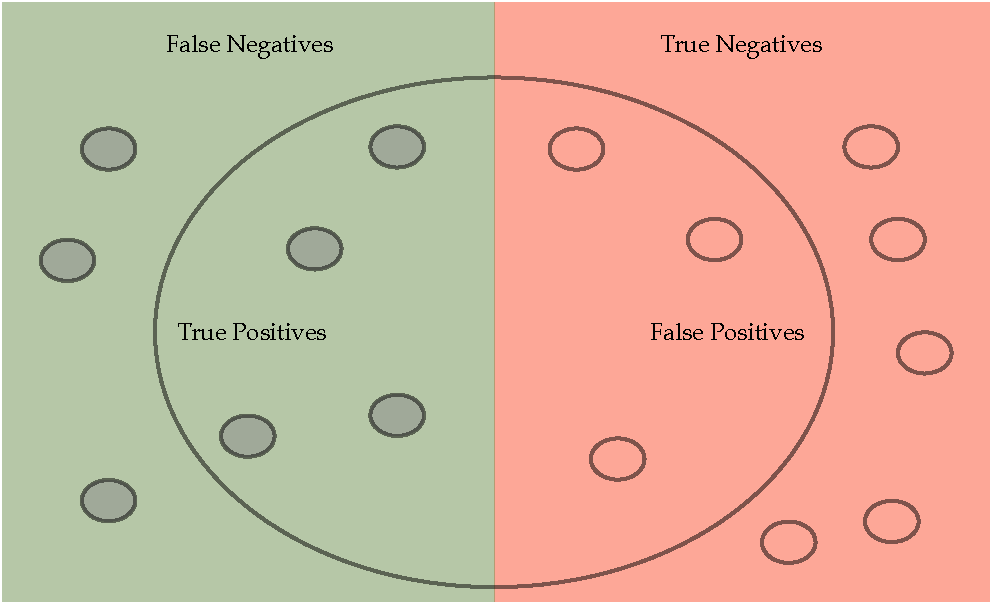
\includegraphics[width=\textwidth]{images/precision-and-recall}
    \caption{Each predicted label \(y_{x}\) is represented by a circle. Hollow circles stand for negative labels and full circles for positive lables.  }
    \label{fig:precision-and-recall}
\end{figure}

The harmonic mean of precision and recall is called \emph{F1-Score} or \emph{F1-Measure}:
\begin{align}\label{eq:f1-score}
\text{F1-Score} = {\left(\frac{Recall^{-1} + Precision^{-1}}{2}\right)}^{-1}
\end{align}
The F1-Score was derived under the name of \emph{MUC-4} by Nancy Chinchor in 1992.~\cite{CHI92}.
Chinchor based her work on the book `Information Retrieval' by Van Rijsbergen from 1979.~\cite{RIJ79}

\subsubsection{Datawig Imputer}
Datawig Imputer is an imputation method based on \emph{supervised learning}.~\cite[p.~1]{BIE18}
It is used in this work for evaluating the robustness of FDs under the name `ML Imputer'.
In the DepDetector algorithm, the Datawig Imputer is used to train models for dependency detection.

The way Datawig Imputer interprets inputs, observations are a set of tuples \( \{\left(\mathbold{x}_1, y_1\right),\left(\mathbold{x}_2, y_2\right), \dots \} \).~\cite[p.~10]{SMO08}
We call \( \mathbold{x}_i \in \mathbb{F}\) \emph{feature-vector} in a \emph{feature-space} \( \mathbb{F} \subseteq \mathbb{R}^{n} \) and \( y_i \in S \) \emph{output-attributes} or \emph{labels}.~\cite[p.~7]{DUD00}

Datawig Imputer solves a classification problem.
A function
\begin{align*}
    f: \mathbb{F} \rightarrow S
\end{align*}
is being approximated, where \( \mathbb{F} \) is the feature-space and \( S = \{a_1, a_2, \dots, a_M \} \) is a set of labels.

Datawig Imputer assumes that the column to be imputed, the so-called \emph{label comumn}, contains data that can be transformed to obtain attributes \( a_1, \dots, a_M \).~\cite[p.~2018]{BIE18}
All columns on a database table that are \emph{not} the label column are called \emph{feature columns}.
These feature columns are transformed by Datawig Imputer to obtain feature-vectors.

The transformation performed to obtain learnable data assign to the \texttt{string} data of each column \( c \) a numerical representation \( x^c \).~\cite[p.~2020]{BIE18}
These functions are called \emph{encoders}.
Datawig Imputer separates data into two categories: \emph{categorical data} and \emph{sequential data}.~\cite[p.~2017]{BIE18}
Different encoders are chosen to transform \emph{categorical data} and \emph{sequential data}.

Categorical data are data that consist of \emph{categorical variables}.
``A categorical variable places a case into one of serveral groups of categories,{''} define Moore et al.\cite[p.~4]{MOO11}
An example-column \( c_{cat} \) containing categorical variables can be representend by the following set of colors:
\begin{align}\label{eq:c-cat}
    c_{cat} = \{ \texttt{blue},~\texttt{red},~\texttt{yellow},~\texttt{blue},~\texttt{blue},~\texttt{red} \}
\end{align}
Datawig Imputer creates a histogram of column \( c \) and uses the histogram's index \( x^c \in \{1, 2, \dots, M_c \} \) to generate a numerical representation.
\begin{figure}[ht]
    \centering
    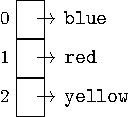
\includegraphics[width=.3\textwidth]{images/state_diagrams/color_histogram}
    \caption{State diagram showing the histogram established by Datawig Imputer to encode example~\ref{eq:c-cat}}
    \label{fig:state-diagram-color}
\end{figure}
Thus the encoded column \( c_{cat} \) would have the following form:
\begin{align*}
    c_{cat}^{c} = \{ 0, 1, 2, 0, 0, 1\}
\end{align*}

Sequential data is data where the sequece in which individual datapoints are stored in contains information.
An example for sequential data would be a column containing non-categorical strings, like Usernames:

\begin{align*}
    c_{seq} = \{ \texttt{ItalyPaleAle},~\texttt{sisou},~\texttt{primos63} \}
\end{align*}

The numerical representation \( c_{seq}^{c} \in \{ 0, 1, 2, \dots, A_c \}^{S_c} \) of the sequential column ``is a vector of length \( S_c \), where \( S_c \) denotes the length of the sequence or \texttt{string} in column \( c_{seq} \).''~\cite[p.~2020]{BIE18}
This numerical representation is called \emph{n-gram representation}.
For further details on the n-gram implementation, consider~\cite[p.~2020]{BIE18}.

Finally, the Datawig-Imputer learns to predict the label distribution from \( y \in {1, 2, \dots, D_y} \) from the feature-vector \( \mathbold{x} \).
It therefore models \( p(y|\mathbold{x},\mathbold{\Theta}) \), the \( D_y \)~-~dimensional probability vector over all possible values in the to-be imputed column in function of feature-vector \( \mathbold{x} \) and \emph{learned model parameters} \( \mathbold{\Theta} \).~\cite[p.~2021]{BIE18}

Datawig uses a logistic regression type output layer to achieve this:
\begin{align*}
    p(y|\mathbold{x},\mathbold{\Theta}) = \texttt{softmax}[\mathbold{Wx} + \mathbold{b}]
\end{align*}
Here, the learned model parameters \( \mathbold{\Theta} = (\mathbold{W}, \mathbold{z}, \mathbold{b}) \) depends on the learned \emph{weights} \( \mathbold{W} \) and \emph{biases} \( \mathbold{b} \) as well as \( \mathbold{z} \), representing all parameters of the column-specific feature extraction.
Parameters \( \mathbold{\Theta} \) are learned by minimizing cross-entropy loss between predicted and observed labels \( y \) by computing
\begin{align}\label{eq:datawig-erm}
    \mathbold{\Theta} = \min_{\Theta} \sum\nolimits_{1}^{N} - \log\left(p\left(y|\mathbold{x}, \mathbold{\Theta}\right)\right)^\top \texttt{onehot}(y).
\end{align}
Here, \( \log() \) represents the element-wise logarithm.
\( \texttt{onehot}(y) \in {0, 1}^{D_y}\) stands for a one-hot encoding of one label \( y \).

Equation~\ref{eq:datawig-erm} is applying the principle of \emph{Empirical Risk Minimization}.~\cite[p.~832]{VAP92}
The right-hand term is the \emph{empirical risk-function} for the classification problem.
By minimizing the risk, in this case cross-entropy loss, weights \( \mathbold{\Theta} \) are `learned' that lead to an optimized classification performance.

Training is done using standard backpropagation and stochastic gradient-descent on mini-batches.
The exact network layout is described in the paper ``Deep Learning for Missing Value imputation in Tables with Non-Numerical Data''~\cite[p.~2022]{BIE18} in full detail.

\subsubsection{ML Imputer}
When Datawig Imputer is employed in the experimental section of this work, it is referred to as `ML Imputer'.
This name is chosen to emphasize the internal mode of operation similar to FD Imputer.
Both imputers use cross-validation to find impute-values on a test set.
They derive either a F1-Score as in equation~\ref{eq:fd-imputer-f1-score} for classifiable data or a MSE as in equation~\ref{eq:fd-imputer-mse}.

\subsection{DepDetector: RFD Discovery}
In the field of data profiling, an extensive body of theory and algorithms for FD discovery has been created in the past decades.~\cite[p.~39]{ABE19}
New techniques such as massive parallelization or hybrid algorithms, combining different discovery strategies, lowered the time needed to detect FDs on a relational table continuously.~\cite[p.~40]{ABE19}

\begin{figure}[ht]
     \centering
     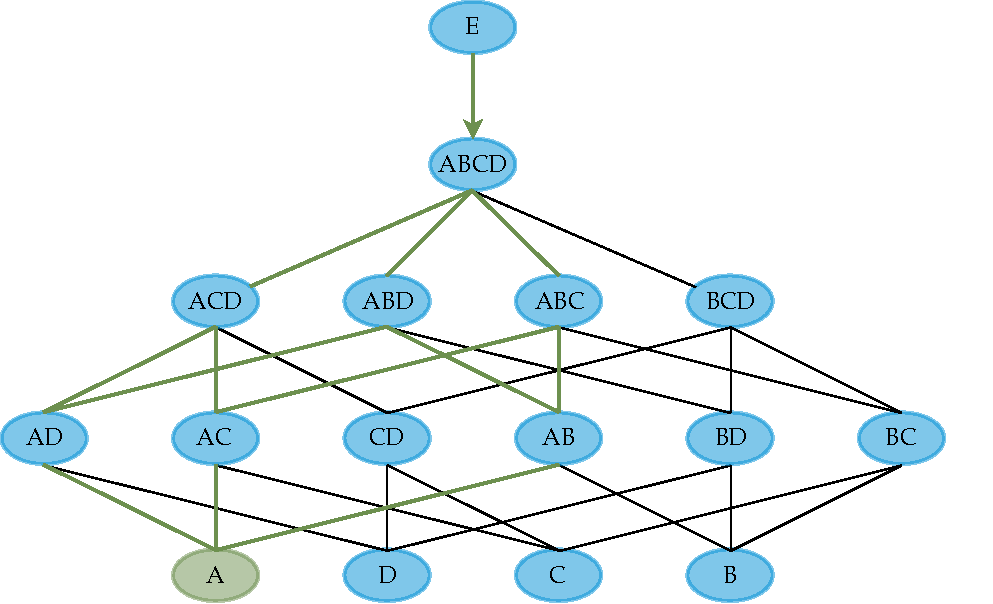
\includegraphics[width=\textwidth]{images/search-lattice-fd.pdf}
     \caption{Hasse diagram of the search lattice when discovering minimal, non-trivial FDs on a relational schema with five columns.}
     \label{fig:dep-detector-search-tree}
 \end{figure}

Notably the \textsc{TANE} algorithm developed by Huhtala et al.\ discovered FDs faster than any other algorithm at the time.~\cite{HUH99}
It paved the way for other algorithms that use the same search strategy called `lattice traversal', such as \textsc{FUN}~\cite{NOV08}, \textsc{FD\_MINE}~\cite{YAO02} and \textsc{DFD}~\cite{ABE14}.~\cite[p.~39]{ABE19}

In an effort to leverage the imputation-capabilities of ML Imputer for dependency discovery, the algorithm called \emph{DepDetector} is introduced.
DepDetector finds RFDs that relax both on the attribute comparison as well as on the extent.
When discovering dependencies, DepDetector searches all non-trivial, minimal dependencies.
Similar to FD discovery algorithms, the search space can be modeled as a graph labeling problem.~\cite[p.~24]{ABE19}
Here, every possible combination of attributes, called \emph{power set} of attribute combinations, from the nodes of the graph.
Due to the properties of the graph, the problem can be modelled as a \emph{lattice}.~\cite[p.~24]{ABE19}
This has been visualized using a Hasse diagram in figure~\ref{fig:dep-detector-search-tree}:
Column \textsc{E} is the RHS for which a minimal LHS is searched.
Green edges visualize paths to the minimal LHS \textsc{A}.
On this path, a number of candidate-LHSs are passed-by.

\subsubsection{DepDetector Algorithm}
DepDetector searches for dependencies by traversing the search lattice as depicted in figure~\ref{fig:dep-detector-search-tree}.
In a first step, ML Imputer is run, imputing the RHS with all other columns on the relational scheme as LHS.
This yields the model's robustness.
For the algorithm to continue traversing the search lattice in search of dependencies, this model's robustness must exceed an initial threshold value.
The threshold value depends on the data type of the potential RHS.
The model is required to either achieve an F1-Score equal or greater than 0.9 or an MSE of less than \( 0.2 \cdot \overline{y} \), where \( \overline{y} \) is the arithmetic mean of all RHS values in the dataset.
If the initial model does not exceed the threshold, we can assume that no dependency is present on the relational instance.

However, if the initial threshold is surpassed, the search-algorithm traverses the search lattice in a `top-down' manner as depicted in figure~\ref{fig:dep-detector-search-tree}.
For each node in the search lattice a model is trained and evaluated.
Again the search is only proceeded, when the model surpasses a threshold: either a smaller MSE than the parent-node, or a F1-Score bigger than 98\% of the parent node's F1-Score.
This is repeated until the threshold is not exceeded by any new model or until a minimal LHS is reached.

\paragraph{DepDetector Relaxing on the Extent}The threshold-driven search-strategy is effectively a relaxation on the extent of the canonical FD when a potential RHS is of a classifiable data type.
It is similar to an AFDs approach of ``holding on almost every tuple'' --- the imputation needs to be correct on almost every instance, but not on every instance.
In addition, ML Imputer is capable of learning conditions, similiar to CFDs.
As shown in the experimental section of this work, ML Imputer learns the order of entries in a relational instance as well as thresholds, such as a CFD\textsuperscript{p} would do.
Compared to CFDs, ECFDs and CFD\textsuperscript{p}s, it is important to keep in mind though that these conditions are never manually set but learned.

The behavior of DepDetector as described in the paragraph above is also displayed in listing~\ref{lst:complete-depdetector}.
Note that DepDetector is implemented with two search-modes called `greeedy' and `complete'.
The `complete' search-mode behaves as described above.
It is optimized to find all dependencies on a relational scheme.
Meanwhile the `greedy' search-mode is optimized to detect just \emph{one} dependency.
This approach converges faster than `complete' and can be used if a single minimal dependency is sufficient.
However, it neither guarantees to find minimal dependencies, nor does it guarantee to find the most robust dependency.

\begin{lstlisting}[caption={`Complete' candidate generation in the DepDetector algorithm},captionpos=b,language=Python,label=lst:complete-depdetector]
def get_complete_candidates(root):
    convergence = True
    most_recent_nodes = root.get_newest_children()
    for node in most_recent_nodes:
        if root.is_continuous:  # sequential data
            if (node.score < node.parent.score) and (len(node.name) > 1):
                convergence = False
                pot_lhs = node.name
                for col in pot_lhs:
                    candidate_lhs = [c for c in pot_lhs if c != col]
                    add_node(candidate_lhs,
                             parent=node,
                             score=None)

        elif not root.is_continuous:  # classifiable data
            if (node.score > node.parent.score*0.98) \
                    and (len(node.name) > 1):
                convergence = False
                pot_lhs = node.name
                for col in pot_lhs:
                    candidate_lhs = [c for c in pot_lhs if c != col]
                    add_node(candidate_lhs,
                             parent=node,
                             score=None)
\end{lstlisting}

\paragraph{DepDetector Relaxing on Attribute Comparison}
A fundamental difference that manifests itself when comparing dependencies discovered by DepDetector with MFDs or FDs is due the fact that DepDetector does not derive the existence of a dependency based on attribute comparison as in equations~\ref{eq:fd-condition}~or~\ref{eq:mfd-condition}.
Instead, DepDetector uses ERM-strategies when executing ML Imputer to measure a dependency's robustness.
Thus, DepDetector optimizes for maximum robustness and a minimum number of LHS attributes.
